In this section, we present the model of the hybrid dynamical system
under test, and the background for PWA relational abstractions.


\subsection{System-under-test ($\System$)}

We assume that the system-under-test is a hybrid dynamical system, \ie, a
system which has discrete modes and a continuous state-space, and which
evolvution is either (1) continuous in time according to the dynamics
associated with its current discrete mode (typically described using
differential equations over its continuous state), or (2) through
discrete jumps that possibly change the discrete mode of the system and
possibly reset its continuous state to some value.  However, we assume
that the system is {\em effectively black-box}. This means that we do not
assume any knowledge of the symbolic dynamical equations describing the
system behavior. We do assume some knowledge of the system: an {\em
interface} view, in which we are allowed to stimulate the system with
inputs and observe its outputs.

We formally define a system-under-test $\System$ as a tuple $(\Modes,
\ContStates, \InitModes, \InitStates, \Delta, \Inputs, \Outputs)$.
Here, system state-space (denoted $\HybridStates$) is a subset of
$\Modes \times \ContStates$, where $\Modes$ is a finite set of
discrete modes, and $\ContStates$ is a compact subset of $\Reals^n$
representing the set of continuous states.  The sets $\InitModes
\subseteq \Modes$ and $\InitStates \subseteq \ContStates$ represent
initial modes and states respectively.  We assume that the system is
{\em initialized} to some initial mode $\initmode \in \InitModes$ and
an initial state $\initstate \in \InitStates$ at time $t=0$.  We
assume that the system has $m$ exogenuous inputs which take values
from the set $\Inputs$ which is a compact subset of $\Reals^m$. We
assume that the system has $\ell \le n$ outputs, where $\Outputs
\subseteq \HybridStates$. In this paper, we assume that the entire
system state is observable.  In other words, $\Outputs =
\HybridStates$.

Finally, we restrict our attention to switched-mode systems, \ie, those in
which there is a partition imposed on $\ContStates$, and there is a
bijective map between each element $\ContStates_i$ in the partition and
each mode in $\Modes$. Thus, we can omit the discrete modes from the
system description, and set $\HybridStates$ = $\ContStates$.

The operational semantics of $\System$ is defined in terms of a {\em
forward simulation map}\footnote{We require that $\System$ can always
be simulated forward in time with deterministic results. A few
technical conditions are required on the system dynamics are required
to ensure that this assumption is valid, see for
example~\cite{Meiss/2007/Differential} and \cite{goebel2012hybrid} for
further details. In practice, such conditions are usually impossible
to check for a black-box model. We then assume that the black-box
model is described as a model in a deterministic simulation framework
such as Simulink\textregistered.} $\simmap_\Delta$, which is a
function that maps a time $t$, the current state of the system, and an
input value in $\Inputs$ to the state of the system at time
$t+\Delta$, \ie, $\simmap_\Delta$ is a function from $\ContStates
\times \Inputs \times \Reals^{\ge 0}$ to $\ContStates$.

% Let $\inputsignal$ = $(t_0, u_0)$, $\ldots$, $(t_N,u_N)$ be a
% timed-sequence of inputs, where $t_0 = 0$, and for all $i > 0$, $t_i -
% t_{i-1} = \Delta$, and $u_i \in \Inputs$.  We can extend the forward
% simulation map to a sequence of states to describe the application of
% an input signal to excite the system as follows:
% $\simmap_\Delta(\initstate, \mathbf{u}) = \contState_N$, if for all $i
% \in [0,N-1]$, $\simmap_\Delta(\contState_i, u_i,t_i) =
% \contState_{i+1}$.
%
% An alternative view of the forward simulation-map is as a
% parameterized reachability relation $\reach_\Delta{t,u} \subseteq
% \ContStates \times \ContStates$ defined as below:
% \[
% (\contState,\contState') \in \reach_\Delta{t,u}\text{ iff } \contState' = \simmap_\Delta(\contState,t,u).
% \]

% inputs modeling an embedded control system.
%
% we assume that the hybrid system is effectively a switched-mode
% dynamical system, \ie, the mode of the system is completely determined
% by its state.  An input to $\System$ is assumed to be a time-bounded
% {\em signal}, \ie, a function from $[0,T]$ to $\Inputs$, with $T$ as
% the time horizon, and $\Inputs \subseteq \Reals^k$.  In this paper, we
% view $\System$ as effectively black-box equipped with a forward
% simulation map, in a simulation time-step of $\Delta_t$ from time $t$,
% allows computing the unique reachable state $\vx \in \HybridStates$
% given state-input pair $(\vx,\vu)$.

% time and input parameterized reachability relation $\reach{t,
% \vu}_\System \subseteq \HybridStates \times \HybridStates$ as follows:
% $\simulate^{\System}:
% (\vx, \vu, t) \mapsto \vx$, where $\vx \in \HybridStates$, $\vu \in
% \Inputs$ and $t \in [0,T]$.


% Given the hybrid state space $\vx\in\HybridStates$ and input space $u
% \in\Inputs$ and time step $t$, it computes the unique successor state
% $\vy=\simulate^{\System}(\vx,u,t)$ such that $\vx \reach{t,u} \vy$.


% \begin{definition}[System Evolution]
%     The behavior of system $\System$ at time $t$ is described as an
%     evolution in the hybrid state-space $\HybridStates$ under the
%     effect of the input $\vu \in \Inputs$ at time $t$. The forward
%     simulation map $\mathsc{sim}^\System : \HybridStates \times \Inputs
%     \times \Reals^+ \mapsto \HybridStates$, maps a state $\x\in\HybridStates$ at time
%     $t$ to a new state $\x'\in\HybridStates$ at time $t+\Delta\in\Reals^+$, under a constant
%     input $\vu$.  Finally, we define the time and input parameterized
%     reachability relation $\reach{t,u} \subseteq \HybridStates \times
%     \HybridStates$ such that
%     \begin{equation}
%         (\vx,\vx') \in \reach{t,u} \;\text{iff}\; \vx'=\mathsc{sim}^{\System}(\vx,u,t).
%     \end{equation}
% \end{definition}

% \mypara{System Assumptions:}
% We require that $\System$ can always be
% simulated forward in time with deterministic results. This in turn
% requires existence and uniqueness of trajectories over a finite time
% horizon $[0,T]$, which can be guaranteed by Lipschitz continuity of
% the vector field in each underlying hybrid mode, ruling away issues
% such as finite escape times~\cite{Meiss/2007/Differential}, and having
% well-defined semantics for simulations at switching boundaries. While
% these assumptions hold for the dynamical system examples which we
% consider in this paper, such assumptions can be restrictive for
% general control system models. When analyzing a system that does not
% obey theoretical conditions that allow deterministic simulation, we
% assume that the underlying tool used for numerical approximations of
% system behaviors uses deterministic simulation semantics.  Finally, we
% assume full observability of the system state, validate our results
% only against the $\mathsc{sim}^\System$ function (as the analytic closed-form
% representation of the system dynamics is assumed to be unavailable).
% From here on, we drop the subscript $\System$ whenever it is clear
% from the context. Also, to ease the presentation, we conflate the
% inputs with the state and denote them by $\vx$.
%
\subsection{$\epsilon$-precision Transition System Abstraction}

We now show how we can abstract a hybrid dynamical system $\System$
which has trajectories in dense-time by a discrete transition system.
A discrete transition system $\mathcal{T}$ can be defined as the tuple
$(\Cells, \CellEdges, \InitCells, \CellLabelingFunction)$, where
$\Cells$ is a finite set of cells, $\CellEdges \subseteq \Cells \times
\Cells$ is an unlabeled transition relation, and
$\CellLabelingFunction$ is a function that assigns one or more labels
to the cells from a finite set $L$ of labels. The operational
semantics of the transition system are as follows: the system starts
in some cell in $\Cells_\init$. At each step, if the transition system
is in cell $C$, it transitions to cell $C'$ if $(C,C') \in
\CellEdges$. A finite-time trace property $\varphi$ of the system is
some subset of the free monoid $(2^L)^*$. We say that $\mathcal{T}
\not\models \varphi$ if there exists some trace of $\mathcal{T}$ such
that the sequence of labels in that trace does not belong to
$\varphi$.

We now give an example of a specific kind of transition system
abstraction that we can build given $\System$ and the simulation map
$\simmap_\Delta$.  We call the transition system an
$\epsilon$-precision transition system ($\epsilon$-TS for short) and
denote it by $\TSAbstraction{\epsilon}{\System}$.  Let $\epsilon  =
10^{-k}$, for some positive integer $k$.  We define a quantization
function $\quant_\epsilon$ that maps a state $\contState$ in
$\ContStates$ to $10^{-k}*\lfloor \contState*10^k \rfloor$. This
transformation essentially truncates the decimal representation of the
numeric value of the state $\state$ to at most $k$ digits after the
decimal point.  This function induces an equivalence relation
$\contState_i \equiv_\epsilon \contState_j$ iff
$\quant_\epsilon(\contState_i) = \quant_\epsilon(\contState_j)$.

Using the equivalence relation $\equiv_\epsilon$, we can now define
the tuple $(\Cells, \CellEdges, \CellLabelingFunction)$ for
$\TSAbstraction{\epsilon}{\System}$ by considering the quotient
structure $\ContStates/\equiv_\epsilon$.  Essentially, each
equivalence class in the quotient structure is a cell in $\Cells$.
For cells $C$ and $C'$ in $\TSAbstraction{\epsilon}{\System}$, the
edge $(C,C')$ can be an element of $\CellEdges$ iff:
$\simmap_\Delta(\contState, u, t)$ = $\contState'$,
$\quant_\epsilon(\contState)$ = $C$, and,
$\quant_\epsilon(\contState') = C'$.

We assume that there is a specified set of states $\UnsafeStates
\subseteq \ContStates$ that are unsafe\footnote{Our framework is
general enough to reason about richer class of correctness properties
for trajectories such as bounded-time LTL properties. In this case, we
assume the LTL property is defined over Boolean-valued predicates over
$\ContStates$. The labeling function $\CellLabelingFunction$ would
then label cells with the predicates that evaluate to $\mathit{true}$
for some state in the cell.}, and thus restrict our attention to
simple safety properties. Thus, our label set has only two elements:
$\setof{\init,\unsafe}$. We then define $\CellLabelingFunction$ as
$\CellLabelingFunction(C) = \init$ if $C$ contains some initial state,
$\CellLabelingFunction(C) = \unsafe$ if $C$ contains some unsafe
state, and empty otherwise.

In what follows, we review the procedure
$\mathsf{ScatterAndSimulate}$($\System$,$\simmap_\Delta$,$\epsilon$)
from \cite{zutshi2014multiple} that, given the $\System$, the forward
simulation map $\simmap_\Delta$, and a precision $\epsilon$ creates an
$\epsilon$-TS abstraction of $\System$.  The
essence of the procedure is a breadth-first exploration of
$\ContStates$ to build $\TSAbstraction{\epsilon}{\System}$ =
$(\Cells,\CellEdges,\CellLabelingFunction)$. It consists of the
following steps:
\begin{enumerate}[leftmargin=1em,labelsep=1em,label={\arabic*.}]
\item
Add a set of random samples from the initial set of states to a queue
(\ie some states $\contState$ at time $0$).
\item
Pop the head of the queue (say state $\contState$ at time $t$), identify
the corresponding cell by applying $\quant_\epsilon$, and add it to
$\Cells$.
\item
Obtain $\contState' = \simmap_\Delta(\contState, t, u)$. Obtain a a
fixed number of states in the neighborhood of $\contState'$, and add
$\contState'$ and these states (all time $t+\Delta$) to the queue.
\item
Add an edge between the cells corresponding to $\contState$ and
$\contState'$.
\item
Go to step 2 till either the queue is empty or a fixed number of cells
or edges is added to $\TSAbstraction{\epsilon}{\System}$.
\end{enumerate}

% \inclfig[width=0.95\linewidth]{vdp_cont_traces.pdf}{Van der
% Pol: continuous trajectories. Red and green boxes indicate unsafe and
% initial sets.}{vdp-cont}
\inclfig[width=0.95\linewidth]{vdp_abs.pdf}{The discovered
$0.2$-TS abstraction. Red cells are unsafe cells and green cells are
initial cells.}{vdp-abs}

\begin{example} 
We now describe $\epsilon$-TS abstraction using the Van der Pol
oscillator benchmark from~\cite{zutshi2014multiple}. Simulations
generated using uniformly random samples are shown in
\figref{vdp-cont}. We want to check the property $P_3$, indicated by
the red box, given the initial set indicated by the green box. We
consider the $\epsilon$-TS abstraction defined by the quantization
function $\quant_{0.2}(\x)$. This results in an evenly gridded
state-space, where each cell is of size $0.2 \times 0.2$ units.
$\mathsf{ScatterAndSimulate}$ is then used to construct
$\TSAbstraction{0.2}{\System}$ using $2$ samples per cell and a time
step of $\Delta = 0.1s$. The complete process follows.  The
$\epsilon$-TS abstraction thus discovered is shown in
\figref{vdp-abs}. The red cells are unsafe and green cells are initial
cells.
\end{example}


% \begin{example}[Van der Pol Oscillator]~\label{ex:vdp}
% 
% \inclfig[width=0.95\linewidth]{vdp_abs.pdf}{The discovered
% abstraction $\epsilon=0.2$. Red cells are unsafe cells and green cells are
% initial cells.}{vdp-abs}
% 
% We use the Van der Pol oscillator benchmark
% from~\cite{zutshi2014multiple} to demonstrate our falsification
% approach. We want to falsify property $P_3$, $x_{unsafe}\in[-1, -6.5]$
% and $y_{unsafe}\in[-0.7, -5.6]$, given the initial set indicated
% $x0\in[-0.4, -0.4],\; y_0\in[0.4, 0.4]$. The abstraction is defined by
% $\epsilon=0.2$, which results in an evenly gridded state-space, where
% each cell is of size $0.2 \times 0.2$ units.  $ScatterAndSimulate$ is
% then used to construct the abstraction, using $2$ samples per cell and
% the time step $\Delta = 0.1s$. The result is plotted in
% ~\figref{vdp-abs}.
% 
% \end{example}

\subsection{CEGAR for falsifying $\TSAbstraction{\epsilon}{\System}$}

We remark that our abstraction is {\em neither an overapproximation
nor an underapproximation} of the continuous-time continuous-space
reachability relation between states. The purpose of the $\epsilon$-TS
is to discover falsifying trajectories. This can be accomplished by
Algorithm~\ref{algo:s3camBMC} that uses CounterExample-Guided
Abstraction and Refinement (CEGAR).

Here, we construct $\TSAbstraction{\epsilon}{\System}$
(Line~\ref{algoline:construct}), we check if there is a path in
$\TSAbstraction{\epsilon}{\System}$ that leads to a cell labeled
unsafe. This can be done by a bounded model checking procedure
(Line~\ref{algoline:bmc}) that explores at most $\ell$ transitions of
$\TSAbstraction{\epsilon}{\System}$ (\ie, traces that are at most
$\ell\Delta$ seconds in length). The model checker may return a set of
counterexample trajectories $\Pi$. If this set is empty
(Line~\ref{algoline:nocex}), then either the exploration performed by
$\mathsf{ScatterAndSimulate}$ is not enough or the system could be
safe. In the former case, the user can increase the scope of
exploration for $\mathsf{ScatterAndSimulate}$.  The next step is to
check if the abstract trajectories are spurious, by performing a
concretization step by performing an actual simulation of the system
(Line~\ref{algoline:checkspurious}). If all abstract counterexample
trajectories are found to be spurious, then
$\TSAbstraction{\epsilon}{\System}$ can be refined, basically by
increasing $\epsilon$.
\begin{algorithm}[t]
\DontPrintSemicolon
\caption{CEGAR for $\TSAbstraction{\epsilon}{\System}$\label{algo:s3camBMC}}
\KwIn{$\System$, $\simmap_\Delta$, $\epsilon_0$ , Smallest Precision $\epsilonmin$}
$\epsilon \assign \epsilon_0$ \;
\While{$\epsilon \ge \epsilonmin$}{
    $\TSAbstraction{\epsilon}{\System}$ $\assign$
    $\mathsf{ScatterAndSimulate}$($\System$,$\simmap_\Delta$,$\epsilon$)
    \nllabel{algoline:construct} \;
    $\Pi$ $\assign$ $\mathsf{BoundedModelCheck}$($\TSAbstraction{\epsilon}{\System}$)
    \nllabel{algoline:bmc} \;
    \lIf {$\Pi = \emptyset$}{ return FAIL \nllabel{algoline:nocex} }
    \lIf {$\mathsf{checkIfConcretizable}(\Pi)$}{ return VIOLATION \nllabel{algoline:checkspurious} }
    $\epsilon$ $\assign$ $\frac{\epsilon}{10}$ \nllabel{algoline:refine} \;
}
\end{algorithm}

The biggest drawback of Algorithm~\ref{algo:s3camBMC} is that with
increasing $\epsilon$, the size of $\Cells$ in
$\TSAbstraction{\epsilon}{\System}$ increases exponentially.  Thus,
every subsequent run of the falsification algorithm is slower. In the
next section, we propose an alternative abstraction that enriches the
basic abstraction proposed here by adding labels to the transitions.
We can then perform refinement by enriching the transition relation,
rather than increasing $\epsilon$.

<<<<<<< HEAD
% \subsection{Example: Van der Pol Oscillator}
% \todo{Takes 4 iterations}
% \inclfig[width=0.90\linewidth]{vdp_disc_map.pdf}{Refinement of
% $\epsilon$-TS.}{vdp-map}
% 
=======
\begin{example}
\inclfig[width=0.90\linewidth]{vdp_disc_map.pdf}{
Abstract trajectories discovered by $ScatterAndSimulate$. Each
    rectangle denotes a cell which is uniquely identified  by the
    tuple against it.
%Cells and trajectory segments used by $1$-relational modeling.
}{vdp-abs-paths}

Going back to the~\exref{vdp}, $ScatterAndSimulate$ is able to
    find several abstract trajectories as shown
    in~\figref{vdp-abs-paths}. However, typically, the refinement by
    increasing the quantization precision requires $4$ refinement
    iterations and finally finds a concrete counter-example for
    $\epsilon=0.125$.
\end{example}


% The abstraction of the hybrid dynamical system is a partitioning of
% the hybrid state space $\HybridStates$ into hyper-rectangles or cells
% $C_i \in \Cells$. The cells are pairwise disjoint $C_i \cap C_j \neq
% \emptyset$ iff $i \neq j$ and their union $\bigcup_{C_i\in\Cells}C_i$
% is the state space $\HybridStates$. The partitions over the continuous
% state space are implicitly defined using a quantization function
% $\quant_\epsilon$ parameterized by the precision $\epsilon$.  This further
% defines an equivalence relations such that $(\vx_i) \equiv (\vx_j)
% \;\text{iff}\; \quant_\epsilon(\vx_i) = \quant_\epsilon(\vx_j)$.  In other
% words, $(\vx_i) \in C_i \; \text{iff} \; C_i = \quant_\epsilon(\vx_i)$. The
% abstraction can be interpreted as a graph and explored using fixed
% time $(\Delta\in\Reals^+)$ relations obtained using
% $\simulate(\vx)$~\footnote{$\simulate(\vx)$ is a fixed
% parameterization of $\mathsc{sim}(\vx,\Delta)$}.
%
% % Such an abstraction is defined by partitioning the
% % state-space of the system using a grid, and hence each abstract state
% % is a hyper-rectangle. The relations between abstract states are
% % obtained by suitably lifting $(\vx,\vx') \in\reach{t,u}$. Considering
% % the abstract states as vertices of a graph and the relations as edges
% % between nodes, the problem of finding an abstract counter-example
% % (CEx) can be cast as finding a path in the graph. Such an abstraction
% % can be explored on-the-fly by enumerating the abstract relations
% % between a pair of states.
%
% \mypara{A discrete abstraction} over a continuous space uses relations
% to describe the behavior of the system over time. Such relations
% abstract the underlying dense-time trajectories of the given dynamical
% system to a transition system.


% relation between concrete states, and concrete
% paths can no longer be constructed directly. Instead, search
% procedures like Counter-Example Guided Refinement (CEGAR) must be used
% to find concrete paths. In general, such search techniques are based
% on refinement of the state-space and exponential with respect to
% computational resources and memory. As an alternative, we introduce
% data driven `enrichment' of abstractions to approximate the concrete
% relations underlying the abstract relations.  Specifically, we use
% linear regression to compute affine maps associated with the relations
% between two abstract states. We then show how associating the computed
% maps with the relations transforms a discrete abstraction into a PWA
% transition system.

% The abstraction of the hybrid dynamical system is a a
% partitioning of the combined state-input space $\HybridStates \times
% \Inputs$ into hyper-rectangles or cells $C_i \in \Cells$. The cells are
% pairwise disjoint $C_i \cap C_j \neq \emptyset$ iff $i \neq j$ and
% their union $\bigcup_{C_i\in\Cells}C_i$ is the state-input
% space $\HybridStates \times \Inputs$. The partitions over
% the continuous input-state space are implicitly defined using a quantization
% function $\quant_\epsilon$ parameterized by the precision $\epsilon$.
% This further defines an equivalence relations such that
% \[
%     (\vx_i, \vu_i) \equiv (\vx_j, \vu_j) \;\text{iff}\; \quant_\epsilon(\vx_i,
%     \vu_i) = \quant_\epsilon(\vx_j, \vu_j)
% \]
% In other words, $(\vx_i, \vu_i) \in C_i \; \text{iff} \; C_i =
% \quant_\epsilon(\vx_i, \vu_i)$.

% \begin{definition}[Graph Abstraction]
%     The quantization function $\quant_\epsilon$ induces a DAG on the discrete
%     abstraction given by a graph $G(V, E)$, where each vertex
%     corresponds to a cell $V_i = C$, and an edge exists between two
%     cells $(C, C') \in E_i$ iff there exist state-input pairs
%     $(\vx,\vu) \in C$, $(\vx', \vu) \in C'$ such that $\vx' =
%     \simulate(\vx, \vu )$.
% \end{definition}


% \begin{definition}[Graph Abstraction]
%     The quantization function $\quant_\epsilon$ induces a directed acyclic
%     graph (DAG) on the discrete
%     abstraction given by a graph $G(V, E)$, where each vertex
%     corresponds to a cell $V_i = C$, and an edge exists between two
%     cells $(C, C') \in E_i$ iff there exist state-input pairs
%     $(\vx) \in C$, $(\vx') \in C'$ such that $\vx' =
%     \simulate(\vx)$.
% \end{definition}
%
%
%
% Given a numerical simulator $\simulate$ and an initial abstraction
% defined by a quantization function $\quant_\epsilon$ and a time step
% $\Delta$, we pick samples and simulate them to explore the abstraction
% on the fly to obtain a graph $G$, which has a finite number of
% abstract states $C$ (or cells) and edges $(C,C')$ iff $C
% \areach{\Delta} C'$.


% \begin{definition}[Abstract State Graph]. Let ∆ > 0 be a fixed time
%     step. The abstract state graph H(∆) for time step ∆ is defined by
%     the set of vertices C, and edges (Ci, Cj ) whenever Ci ∆ Cj . Let
%     C0 denote the collection of initial cells in C, i.e., cells Ci
%     such that Ci ∩ X0 6= ∅. Further, let Cu denote the set of unsafe
%     cells, or cells Cj such that there is a state xj ∈ Cj that reaches
%     an unsafe state y ∈ Xf within time 0 ≤ tj < ∆. The abstraction
% H(∆) is given by D C, ∆ , C0, Cu E .  \end{definition}


% As
% Instead of using a CEGAR like loop (used in~\cite{zutshi2014multiple}),
% we use the generated trajectories to learn quantitative models
% describing the local behavior of the system. These models are defined
% by a set of relations $R \subseteq \HybridStates \times \HybridStates$
% for each edge of the reachability graph. In the next section, we
% summarize this idea.


% \subsection{Enriched Abstraction}
%
% 
\begin{figure}[!htbp]
\begin{center}
\tikzstyle{line} = [thick]
\tikzstyle{arw} = [->, thick,>=stealth,shorten <=2pt, shorten >=2pt]
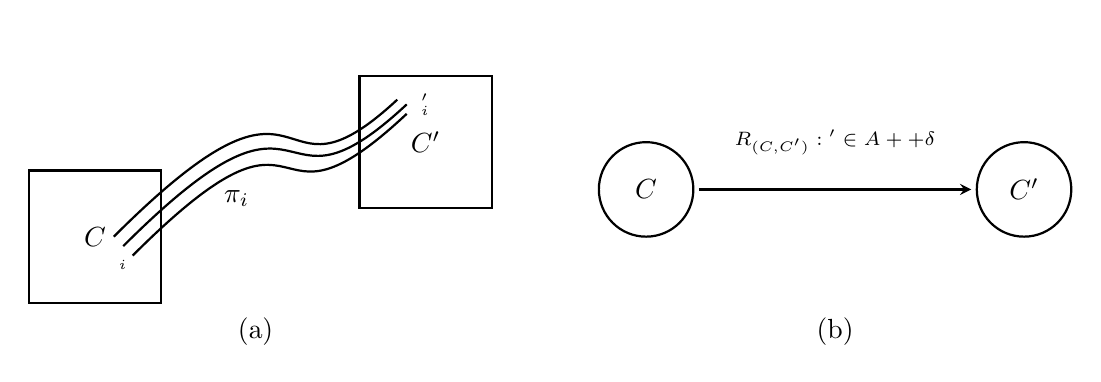
\begin{tikzpicture}
\begin{scope}[scale=1.2]

    \draw [line] (-5.2,-1.2) rectangle (-3.8,0.2);
    \draw [line] (-1.7,-0.2) rectangle (-0.3,1.2);
    \draw [line] (-4.1,-0.7) .. controls +(2.0,2.0) and +(-1.6,-1.5) ..  (-1.2,0.8);
    \draw [line] (-4.2,-0.6) .. controls +(2.1,2.1) and +(-1.5,-1.4) ..  (-1.2,0.9);
    \draw [line] (-4.3,-0.5) .. controls +(2.2,2.2) and +(-1.4,-1.3) ..  (-1.3,0.95);

\node at (-4.5, -0.5) {$C$};
\node at (-1, 0.5) {$C'$};
\node at (-4.2,-0.8) {\scriptsize{$\x_i$}};
\node at (-1.0,0.90) {\scriptsize{$\x_i'$}};
\node at (-3,-0.1) {$\pi_i$};
\node at (-2.8, -1.5) {(a)};
\end{scope}

\begin{scope}[xshift=4.0cm,scale=1.2]
\draw [line] (-2.0,0) circle (0.5);
\draw [line] (2.0,0) circle (0.5);
\draw[arw] (-1.5,0) -- (1.5,0);
\node at (-2.0,0) {$C$};
\node at (2.0,0) {$C'$};
\node at (0,0.5) {\scriptsize{$R_{(C,C')}:\setof{\x' \in A\x + \vb + \delta}$}};
\node at (0.,-1.5) {(b)};
\end{scope}
\end{tikzpicture}
\end{center}
\vspace*{-.3cm}
\caption{(a) Trajectory segments $\traj_i$ are used to compute the
relation $R_{(C,C')}$ that annotates the edge in (b).
$R_{(C,C')}:\setof{\x' \in A\x + \vb + \delta}$ is an interval affine
relation defined by an affine map (matrix $A$ and vector $\vb$) and an
error interval (vector of intervals $\delta$).}
    \label{fig:enriched-edge}
\vspace*{-.3cm}
 \end{figure}

%
% Recall that each edge $(C,C')$ of the graph $G$ denotes an observed
% trajectory between the respective cells. The graph abstraction $G$
% only states that there exists a state $\x \in C$ from which the system
% can evolve to a future state $\x' \in C'$. To increase the precision,
% iterative refinement of the abstraction by state splitting was
% proposed in~\cite{zutshi2014multiple}. Due to the curse of
% dimensionality, state splitting is not scalable. Instead, we propose
% an `enrichment' $G^R$ of $G$ by computing a set of local relations
% $R_{(C,C')}(\x,\x')$ for every edge $(C,C')$, which
% non-deterministically describe relations between $\x \in C$ and $\x'
% \in C'$. This is illustrated in \figref{enriched-edge}.
% %(compare with \figref{segtraj}).
%
% The enriched graph $G^R$ captures the underlying local forward
% dynamics describing the evolution of the system in each abstract
% state. We represent the dynamics using an affine model with an
% interval error. Such a model can either be approximated using learning
% methods or computed as a sound (over) approximation using reachability
% set computation methods. Because we assume black box semantics, we
% only present the former. Using regression analysis on a witnessed
% trajectory between two cells, we compute an approximate discrete map
% along with an error estimate.  Moreover, using the simulation function
% $\simulate$, additional trajectories (or data) can be generated if
% required. The data can be separated into a training set and testing
% set to compute the map and the error respectively.
%
% %The latter case can be explored if
% %the symbolic dynamics of the system are known. A tool like
% %\flowstar~\cite{chen2013flow} can be used to find the reachable set
% %map.
%
% Observe that $G^R$, a directed reachability graph, is rich enough to
% search for concrete behaviors in the system. We call it a time
% parameterized PWA relational abstraction. It can be interpreted as an
% infinite state discrete transition system, and we can use
% off-the-shelf bounded model checkers to find concrete violations of a
% given safety property, and even other temporal properties.

% \begin{figure}[!htbp]
% \begin{center}
% \tikzstyle{line} = [thick]
% \tikzstyle{arw} = [->, thick,>=stealth,shorten <=2pt, shorten >=2pt]
% \tikzstyle{block} = [rectangle, minimum width=0.5cm, minimum height=1.0cm, text centered, draw=black, align=center]%, fill=blue!25]
% \begin{tikzpicture}[scale=1.0, on grid, auto]
%
%     \node (G) at (-4,0) {$G$};
%     \node (GR) at (0,0) {$G^R$};
%     \node (CEX) at (4,0) {$CEx$};
%
%     \node (enrich) [block] at (-2, 0) {\scriptsize Enrich using \\ \scriptsize affine  maps};
%     \node (BMC) [block] at (2, 0) {\scriptsize Find CEx \\ \scriptsize using BMC};
%
%     %\node[align=center] at (0, 0) {\scriptsize Enrich using \\ \scriptsize Regression \\ \scriptsize(OLS)};
%
%     %\draw [line] (-2.0,-0.5) rectangle (-1.0,0.5);
%     \draw[arw] (G.east) -- (enrich.west);
%     \draw[arw] (enrich.east) -- (GR.west);
%     \draw[arw] (GR.east) -- (BMC.west);
%     \draw[arw] (BMC.east) -- (CEX.west);
%
% \end{tikzpicture}
% \end{center}
% \vspace*{-.3cm}
% \caption{Finding counter-examples (CEx) in a graph abstraction using PWA models.}
% \label{fig:overview}
% \vspace*{-.3cm}
% \end{figure}
>>>>>>> 616701974fe662da2ab3292e6ba97f90cf8bcb1c
